% Created by tikzDevice version 0.9 on 2016-01-25 21:33:12
% !TEX encoding = UTF-8 Unicode
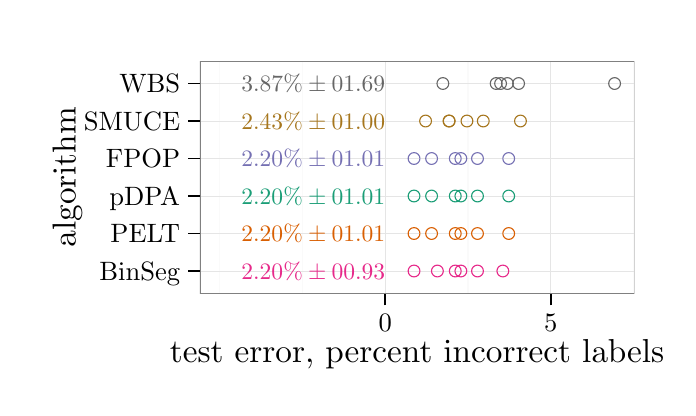
\begin{tikzpicture}[x=1pt,y=1pt]
\definecolor{fillColor}{RGB}{255,255,255}
\path[use as bounding box,fill=fillColor,fill opacity=0.00] (0,0) rectangle (231.26,130.09);
\begin{scope}
\path[clip] (  0.00,  0.00) rectangle (231.26,130.09);
\definecolor{drawColor}{RGB}{255,255,255}
\definecolor{fillColor}{RGB}{255,255,255}

\path[draw=drawColor,line width= 0.6pt,line join=round,line cap=round,fill=fillColor] (  0.00, -0.00) rectangle (231.26,130.09);
\end{scope}
\begin{scope}
\path[clip] ( 62.21, 34.03) rectangle (219.22,118.04);
\definecolor{fillColor}{RGB}{255,255,255}

\path[fill=fillColor] ( 62.21, 34.03) rectangle (219.22,118.04);
\definecolor{drawColor}{gray}{0.98}

\path[draw=drawColor,line width= 0.6pt,line join=round] ( 69.35, 34.03) --
	( 69.35,118.04);

\path[draw=drawColor,line width= 0.6pt,line join=round] ( 99.27, 34.03) --
	( 99.27,118.04);

\path[draw=drawColor,line width= 0.6pt,line join=round] (159.10, 34.03) --
	(159.10,118.04);

\path[draw=drawColor,line width= 0.6pt,line join=round] (218.94, 34.03) --
	(218.94,118.04);
\definecolor{drawColor}{gray}{0.90}

\path[draw=drawColor,line width= 0.2pt,line join=round] ( 62.21, 42.16) --
	(219.22, 42.16);

\path[draw=drawColor,line width= 0.2pt,line join=round] ( 62.21, 55.71) --
	(219.22, 55.71);

\path[draw=drawColor,line width= 0.2pt,line join=round] ( 62.21, 69.26) --
	(219.22, 69.26);

\path[draw=drawColor,line width= 0.2pt,line join=round] ( 62.21, 82.81) --
	(219.22, 82.81);

\path[draw=drawColor,line width= 0.2pt,line join=round] ( 62.21, 96.36) --
	(219.22, 96.36);

\path[draw=drawColor,line width= 0.2pt,line join=round] ( 62.21,109.91) --
	(219.22,109.91);

\path[draw=drawColor,line width= 0.2pt,line join=round] (129.19, 34.03) --
	(129.19,118.04);

\path[draw=drawColor,line width= 0.2pt,line join=round] (189.02, 34.03) --
	(189.02,118.04);
\definecolor{drawColor}{RGB}{231,41,138}

\node[text=drawColor,anchor=base east,inner sep=0pt, outer sep=0pt, scale=  0.85] at (129.19, 39.24) {$2.20\% \pm 00.93$};
\definecolor{drawColor}{RGB}{217,95,2}

\node[text=drawColor,anchor=base east,inner sep=0pt, outer sep=0pt, scale=  0.85] at (129.19, 52.79) {$2.20\% \pm 01.01$};
\definecolor{drawColor}{RGB}{27,158,119}

\node[text=drawColor,anchor=base east,inner sep=0pt, outer sep=0pt, scale=  0.85] at (129.19, 66.33) {$2.20\% \pm 01.01$};
\definecolor{drawColor}{RGB}{117,112,179}

\node[text=drawColor,anchor=base east,inner sep=0pt, outer sep=0pt, scale=  0.85] at (129.19, 79.88) {$2.20\% \pm 01.01$};
\definecolor{drawColor}{RGB}{166,118,29}

\node[text=drawColor,anchor=base east,inner sep=0pt, outer sep=0pt, scale=  0.85] at (129.19, 93.43) {$2.43\% \pm 01.00$};
\definecolor{drawColor}{gray}{0.40}

\node[text=drawColor,anchor=base east,inner sep=0pt, outer sep=0pt, scale=  0.85] at (129.19,106.98) {$3.87\% \pm 01.69$};
\definecolor{drawColor}{RGB}{231,41,138}

\path[draw=drawColor,line width= 0.4pt,line join=round,line cap=round] (154.51, 42.16) circle (  2.13);

\path[draw=drawColor,line width= 0.4pt,line join=round,line cap=round] (162.54, 42.16) circle (  2.13);

\path[draw=drawColor,line width= 0.4pt,line join=round,line cap=round] (139.61, 42.16) circle (  2.13);

\path[draw=drawColor,line width= 0.4pt,line join=round,line cap=round] (156.53, 42.16) circle (  2.13);

\path[draw=drawColor,line width= 0.4pt,line join=round,line cap=round] (148.05, 42.16) circle (  2.13);

\path[draw=drawColor,line width= 0.4pt,line join=round,line cap=round] (171.70, 42.16) circle (  2.13);
\definecolor{drawColor}{RGB}{217,95,2}

\path[draw=drawColor,line width= 0.4pt,line join=round,line cap=round] (154.51, 55.71) circle (  2.13);

\path[draw=drawColor,line width= 0.4pt,line join=round,line cap=round] (162.54, 55.71) circle (  2.13);

\path[draw=drawColor,line width= 0.4pt,line join=round,line cap=round] (139.61, 55.71) circle (  2.13);

\path[draw=drawColor,line width= 0.4pt,line join=round,line cap=round] (156.53, 55.71) circle (  2.13);

\path[draw=drawColor,line width= 0.4pt,line join=round,line cap=round] (145.95, 55.71) circle (  2.13);

\path[draw=drawColor,line width= 0.4pt,line join=round,line cap=round] (173.82, 55.71) circle (  2.13);
\definecolor{drawColor}{RGB}{27,158,119}

\path[draw=drawColor,line width= 0.4pt,line join=round,line cap=round] (154.51, 69.26) circle (  2.13);

\path[draw=drawColor,line width= 0.4pt,line join=round,line cap=round] (162.54, 69.26) circle (  2.13);

\path[draw=drawColor,line width= 0.4pt,line join=round,line cap=round] (139.61, 69.26) circle (  2.13);

\path[draw=drawColor,line width= 0.4pt,line join=round,line cap=round] (156.53, 69.26) circle (  2.13);

\path[draw=drawColor,line width= 0.4pt,line join=round,line cap=round] (145.95, 69.26) circle (  2.13);

\path[draw=drawColor,line width= 0.4pt,line join=round,line cap=round] (173.82, 69.26) circle (  2.13);
\definecolor{drawColor}{RGB}{117,112,179}

\path[draw=drawColor,line width= 0.4pt,line join=round,line cap=round] (154.51, 82.81) circle (  2.13);

\path[draw=drawColor,line width= 0.4pt,line join=round,line cap=round] (162.54, 82.81) circle (  2.13);

\path[draw=drawColor,line width= 0.4pt,line join=round,line cap=round] (139.61, 82.81) circle (  2.13);

\path[draw=drawColor,line width= 0.4pt,line join=round,line cap=round] (156.53, 82.81) circle (  2.13);

\path[draw=drawColor,line width= 0.4pt,line join=round,line cap=round] (145.95, 82.81) circle (  2.13);

\path[draw=drawColor,line width= 0.4pt,line join=round,line cap=round] (173.82, 82.81) circle (  2.13);
\definecolor{drawColor}{RGB}{166,118,29}

\path[draw=drawColor,line width= 0.4pt,line join=round,line cap=round] (158.73, 96.36) circle (  2.13);

\path[draw=drawColor,line width= 0.4pt,line join=round,line cap=round] (164.63, 96.36) circle (  2.13);

\path[draw=drawColor,line width= 0.4pt,line join=round,line cap=round] (143.78, 96.36) circle (  2.13);

\path[draw=drawColor,line width= 0.4pt,line join=round,line cap=round] (152.32, 96.36) circle (  2.13);

\path[draw=drawColor,line width= 0.4pt,line join=round,line cap=round] (152.24, 96.36) circle (  2.13);

\path[draw=drawColor,line width= 0.4pt,line join=round,line cap=round] (178.07, 96.36) circle (  2.13);
\definecolor{drawColor}{gray}{0.40}

\path[draw=drawColor,line width= 0.4pt,line join=round,line cap=round] (169.29,109.91) circle (  2.13);

\path[draw=drawColor,line width= 0.4pt,line join=round,line cap=round] (170.88,109.91) circle (  2.13);

\path[draw=drawColor,line width= 0.4pt,line join=round,line cap=round] (150.03,109.91) circle (  2.13);

\path[draw=drawColor,line width= 0.4pt,line join=round,line cap=round] (173.35,109.91) circle (  2.13);

\path[draw=drawColor,line width= 0.4pt,line join=round,line cap=round] (177.39,109.91) circle (  2.13);

\path[draw=drawColor,line width= 0.4pt,line join=round,line cap=round] (212.08,109.91) circle (  2.13);
\definecolor{drawColor}{gray}{0.50}

\path[draw=drawColor,line width= 0.6pt,line join=round,line cap=round] ( 62.21, 34.03) rectangle (219.22,118.04);
\end{scope}
\begin{scope}
\path[clip] (  0.00,  0.00) rectangle (231.26,130.09);
\definecolor{drawColor}{RGB}{0,0,0}

\node[text=drawColor,anchor=base east,inner sep=0pt, outer sep=0pt, scale=  0.96] at ( 55.10, 38.86) {BinSeg};

\node[text=drawColor,anchor=base east,inner sep=0pt, outer sep=0pt, scale=  0.96] at ( 55.10, 52.41) {PELT};

\node[text=drawColor,anchor=base east,inner sep=0pt, outer sep=0pt, scale=  0.96] at ( 55.10, 65.96) {pDPA};

\node[text=drawColor,anchor=base east,inner sep=0pt, outer sep=0pt, scale=  0.96] at ( 55.10, 79.51) {FPOP};

\node[text=drawColor,anchor=base east,inner sep=0pt, outer sep=0pt, scale=  0.96] at ( 55.10, 93.06) {SMUCE};

\node[text=drawColor,anchor=base east,inner sep=0pt, outer sep=0pt, scale=  0.96] at ( 55.10,106.61) {WBS};
\end{scope}
\begin{scope}
\path[clip] (  0.00,  0.00) rectangle (231.26,130.09);
\definecolor{drawColor}{RGB}{0,0,0}

\path[draw=drawColor,line width= 0.6pt,line join=round] ( 57.95, 42.16) --
	( 62.21, 42.16);

\path[draw=drawColor,line width= 0.6pt,line join=round] ( 57.95, 55.71) --
	( 62.21, 55.71);

\path[draw=drawColor,line width= 0.6pt,line join=round] ( 57.95, 69.26) --
	( 62.21, 69.26);

\path[draw=drawColor,line width= 0.6pt,line join=round] ( 57.95, 82.81) --
	( 62.21, 82.81);

\path[draw=drawColor,line width= 0.6pt,line join=round] ( 57.95, 96.36) --
	( 62.21, 96.36);

\path[draw=drawColor,line width= 0.6pt,line join=round] ( 57.95,109.91) --
	( 62.21,109.91);
\end{scope}
\begin{scope}
\path[clip] (  0.00,  0.00) rectangle (231.26,130.09);
\definecolor{drawColor}{RGB}{0,0,0}

\path[draw=drawColor,line width= 0.6pt,line join=round] (129.19, 29.77) --
	(129.19, 34.03);

\path[draw=drawColor,line width= 0.6pt,line join=round] (189.02, 29.77) --
	(189.02, 34.03);
\end{scope}
\begin{scope}
\path[clip] (  0.00,  0.00) rectangle (231.26,130.09);
\definecolor{drawColor}{RGB}{0,0,0}

\node[text=drawColor,anchor=base,inner sep=0pt, outer sep=0pt, scale=  0.96] at (129.19, 20.31) {0};

\node[text=drawColor,anchor=base,inner sep=0pt, outer sep=0pt, scale=  0.96] at (189.02, 20.31) {5};
\end{scope}
\begin{scope}
\path[clip] (  0.00,  0.00) rectangle (231.26,130.09);
\definecolor{drawColor}{RGB}{0,0,0}

\node[text=drawColor,anchor=base,inner sep=0pt, outer sep=0pt, scale=  1.20] at (140.72,  9.03) {test error, percent incorrect labels};
\end{scope}
\begin{scope}
\path[clip] (  0.00,  0.00) rectangle (231.26,130.09);
\definecolor{drawColor}{RGB}{0,0,0}

\node[text=drawColor,rotate= 90.00,anchor=base,inner sep=0pt, outer sep=0pt, scale=  1.20] at ( 17.30, 76.04) {algorithm};
\end{scope}
\end{tikzpicture}
